\documentclass[11pt]{article}
\usepackage[T1]{fontenc}
\usepackage[utf8]{inputenc}
\usepackage{lmodern,amsmath,amssymb,graphicx,geometry,microtype,setspace,booktabs,caption}
\usepackage[hidelinks]{hyperref}
\geometry{letterpaper,margin=1in}
\setlength{\parindent}{0pt}
\setlength{\parskip}{0.55em}
\setlength{\emergencystretch}{2em}
\captionsetup{labelfont=bf,font=small}
\renewcommand{\refname}{References}
\pagestyle{empty}
\renewcommand{\thefigure}{S\arabic{figure}}
\setcounter{figure}{14}
\begin{document}
\begin{figure}[!ht]\centering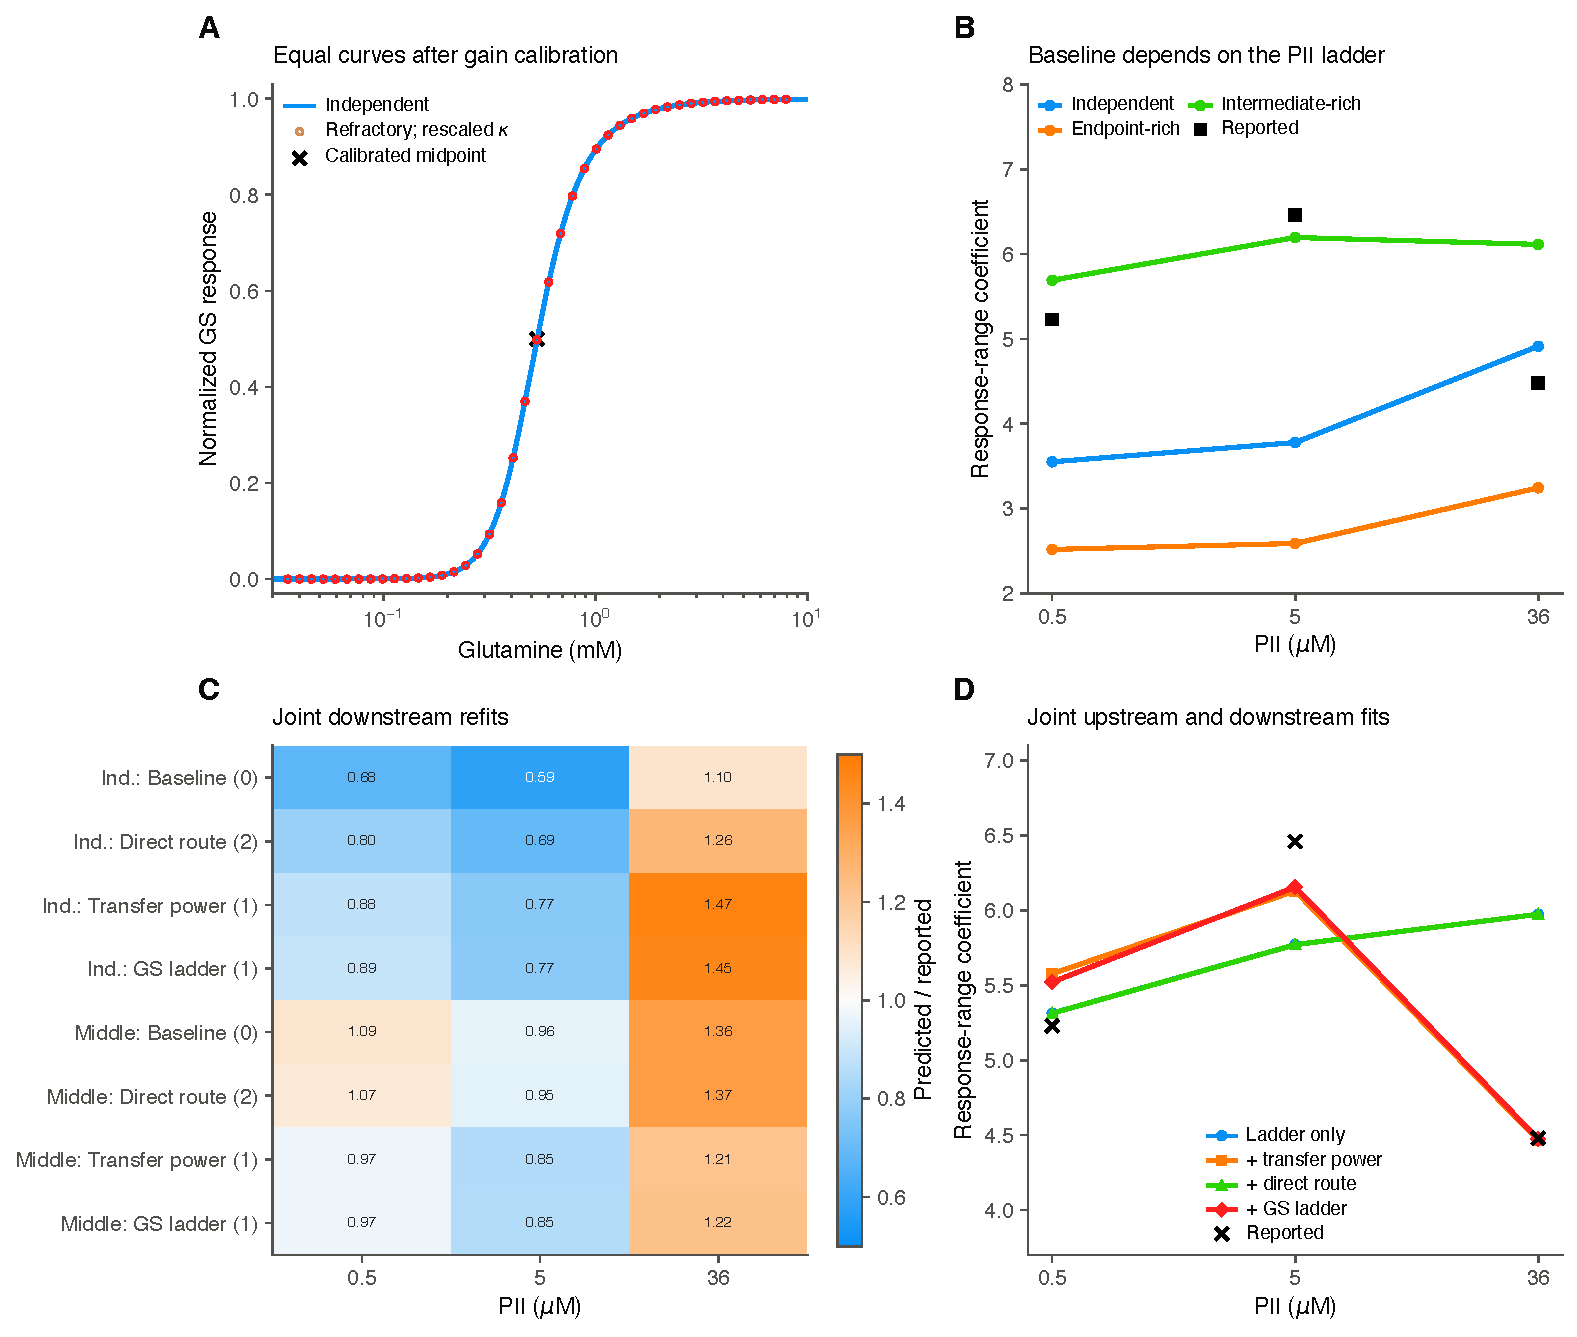
\includegraphics[width=\textwidth,height=0.60\textheight,keepaspectratio]{figure_inputs/FigS15_extended.pdf}\caption{\textbf{Matched calibration separates observational equivalence from model-dependent discrepancy.} (A) Identical independent-population and refractory-population cascade curves after gain rescaling, shown at the middle-condition midpoint. Curves are predictions; the cross is a calibration target. (B) Baseline response-range predictions from three exact mean-matched ladders and reported summaries. (C) Predicted-to-reported ratios after joint fitting for fixed independent or intermediate-enriched PII ladders. Parentheses give the number of added shared downstream parameters; all models also use three condition-specific midpoint gains. (D) Joint comparisons allowing one additional shared upstream ladder parameter. The transfer-power model is a phenomenological benchmark. No summary errors are available for likelihood-based selection. Smooth lines connect the three assay conditions and do not establish a concentration law.}


\end{figure}
\end{document}
